\section{Lernziele (Leitfragen) SW 06}
\begin{itemize}
    \item Wie finde ich meine IPv4 Konfiguration?
    \item Wie finde ich eine IP-Adresse in Verbindung zu einer URL?
    \item Wie finde ich heraus, ob ein Host anhand seiner IP oder URL verfügbar ist?
    \item Wie finde ich heraus, welche Intermediate Network Devices sich zwischen meinem und einem anderen Host befinden, vorausgesetzt es ist eine IPv4 Adresse oder URL?
    \item Wieso brauchen wir IPv6? Was sind die Nachteile von IPv4?
    \item Wie lange sind IPv6 Adressen?
    \item Was sind die Regeln, um eine IPv6 Adresse zu komprimieren?
    \item Wie sind IPv6 Adressen unterteilt?
    \item Was für IPv6 unicast Adress Arten gibt es?
    \item Über welche IPv6 unicast Adressen sollte ein richtig konfigurierte Host mindestens verfügen?
    \item Wie sind IPv6 Global Unicast Addresses (GUAs) unterteilt?
    \item Welche Mechanismen werden verwendet, um IPv4 und IPv6 Netzwerken miteinander zu verbinden?
\end{itemize}

\section{Antworten}
\subsection*{Wie finde ich meine IPv4 Konfiguration?}
\begin{multicols}{2}
    Windows: \texttt{ipconfig [/all]}
    \begin{figure}[H]
        \begin{center}
        \label{pic:ipconfig}
        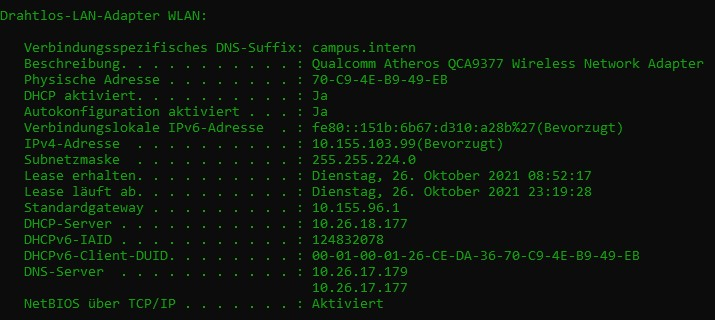
\includegraphics[width=.5\textwidth]{images/ipconfig.jpg}
        \caption{Adapterkonfiguration in Windows mit \texttt{ipconfig /all}}
        \end{center}
    \end{figure}
    \columnbreak
    Unix: \texttt{ifconfig}
    \begin{figure}[H]
        \begin{center}
        \label{pic:ifconfig}
        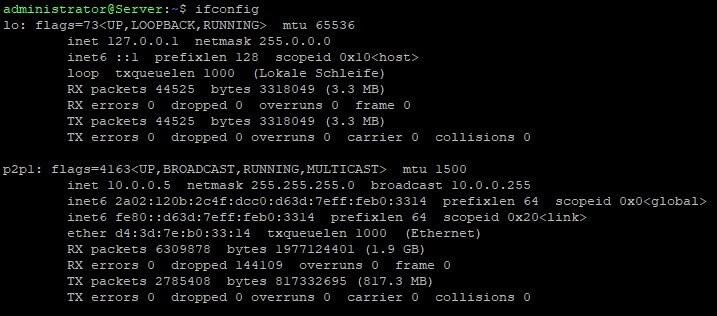
\includegraphics[width=.5\textwidth]{images/ifconfig.jpg}
        \caption{Adapterkonfiguration in Ubuntu mit \texttt{ifconfig}}
        \end{center}
    \end{figure}
\end{multicols}

\subsection*{Wie finde ich eine IP-Adresse in Verbindung zu einer URL?}
\begin{multicols}{2}
    \texttt{nslookup <URL>}
    \begin{figure}[H]
        \begin{center}
        \label{pic:nslookup_win{Sprungmarke}}
        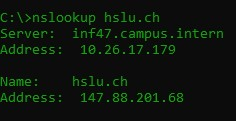
\includegraphics[width=.5\textwidth]{images/nslookup_win.jpg}
        \caption{\texttt{nslookup} in Windows}
        \end{center}
    \end{figure}
    \columnbreak
    \vfill\null
    \begin{figure}[H]
        \begin{center}
        \label{pic:nslookup_unix}
        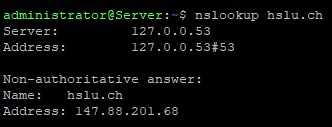
\includegraphics[width=.5\textwidth]{images/nslookup_unix.jpg}
        \caption{\texttt{nslookup} in Ubuntu}
        \end{center}
    \end{figure}
\end{multicols}

\pagebreak
\subsection*{Wie finde ich heraus, ob ein Host anhand seiner IP oder URL verfügbar ist?}
\begin{multicols}{2}
    Windows:
    \begin{itemize}
        \item \texttt{ping [-4] <URL>}
        \item \texttt{ping <IPv4-Adresse>}
    \end{itemize}
    \begin{figure}[H]
        \begin{center}
        \label{pic:ping_win}
        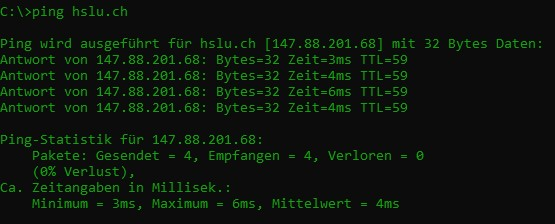
\includegraphics[width=.5\textwidth]{images/ping_win.jpg}
        \caption{\texttt{ping} in Windows}
        \end{center}
    \end{figure}
    \columnbreak
    Unix: \texttt{ping <IPv4-Adresse | URL>} (Ctrl+C zum abbrechen)
    \vfill\null
    \begin{figure}[H]
        \begin{center}
        \label{pic:ping_unix}
        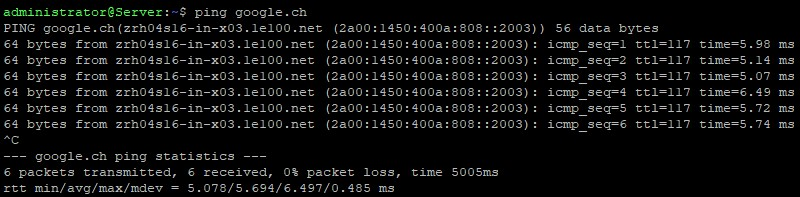
\includegraphics[width=.5\textwidth]{images/ping_unix.jpg}
        \caption{\texttt{ping} in Ubuntu}
        \end{center}
    \end{figure}
\end{multicols}

\subsection*{Wie finde ich heraus, welche Intermediate Network Devices sich zwischen meinem und einem anderen Host befinden, vorausgesetzt es ist eine IPv4 Adresse oder URL?}
\begin{multicols}{2}
    Windows:
    \begin{itemize}
        \item \texttt{tracert [-4] <URL>}
        \item \texttt{tracert <IPv4 Address>}
    \end{itemize}
    \begin{figure}[H]
        \begin{center}
        \label{pic:tracert}
        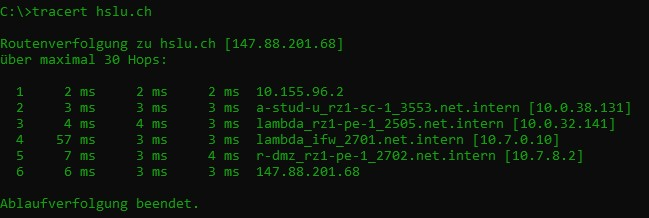
\includegraphics[width=.5\textwidth]{images/tracert.jpg}
        \caption{\texttt{tracert} in Windows}
        \end{center}
    \end{figure}
    %\vfill\null
    \columnbreak
    Unix: \texttt{traceroute <IPv4 Adress | URL>}
    \begin{figure}[H]
        \begin{center}
        \label{pic:traceroute}
        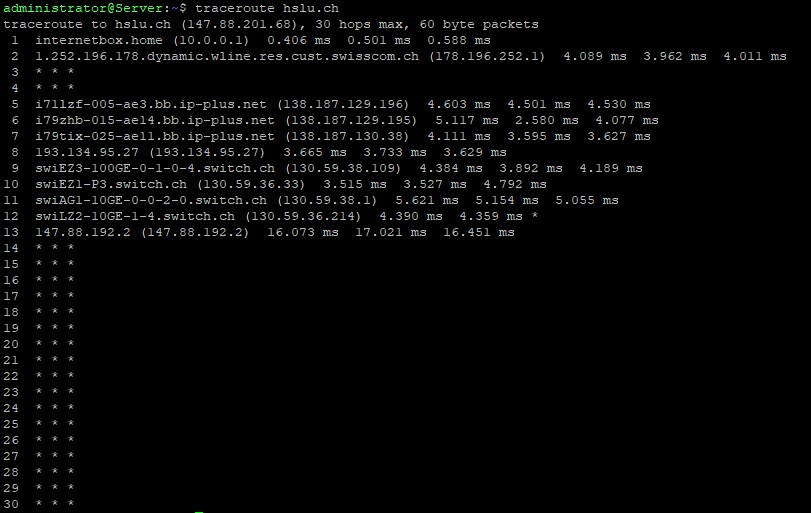
\includegraphics[width=.5\textwidth]{images/traceroute.jpg}
        \caption{\texttt{traceroute} in Ubuntu}
        \end{center}
    \end{figure}
\end{multicols}

\subsection*{Wieso brauchen wir IPv6? Was sind die Nachteile von IPv4?}
Auf die Länge von 32 bits gibt es lediglich $2^{32}=4'228'250'625$ IPv4 Adressen. Vergleichsweise weniger als die Hälfte der Weltbevölkerung. Es kommt deshalb zu einem Engpass an verfügbaren öffentlichen IPv4 Adressen. IPv6 mit 128 bits hat $2^{128}=3.4\times10^{38}$. Das ist viel mehr als die geschätzte Anzahl Sandkörner auf der Erde ($6.63\times10^{22}$\footnote{\url{https://www.why.is/svar.php?id=4803}}) oder Galaxien im Universum ($10^{22}$ - $10^{24}$\footnote{\url{https://www.esa.int/Science_Exploration/Space_Science/Herschel/How_many_stars_are_there_in_the_Universe}}

\subsection*{Wie lange sind IPv6 Adressen?}
16 bytes = 128 bits, wie bereits erwähnt.

\subsection*{Was sind die Regeln, um eine IPv6 Adresse zu komprimieren?}
Es werden möglichst alle (führenden) Nullen komprimiert. Sind mehrere Hextete (vier Hexadezimalwerte) hintereinander nullen, so fasst man es mit einem doppelten Doppelpunkt (::) zusammen. Dies ist aber nur einmal möglich!

\begin{tabularx}{\textwidth}{lX}
    Typ&Format\\
    \hline
    Normal&\texttt{2001:{\color{green}0000}:{\color{green}0000}:1111:{\color{magenta}0000}:{\color{magenta}0000}:{\color{magenta}0000}:{\color{magenta}0}200}\\
    Komprimiert&\texttt{2001:{\color{green}0}:{\color{green}0}:1111{\color{magenta}::}200}
\end{tabularx}

\subsection*{Wie sind IPv6 Adressen unterteilt?}
Die Präfixlänge ist in der \textsl{Slash Notation} geschrieben und zeigt den Netzwerk Teil der IPv6 Adresse an. Die Präfixlänge kann von 0 bis 128 gehen. Allgemein wird eine Präfixlänge von /64 empfohlen.\\

Nachfolgend ein Beispiel für \texttt{2001:db8:a::/64}\\[1em]
\begin{tabular}{ccc}
    \multicolumn{1}{c}{64 bits}&\multicolumn{1}{c}{}&\multicolumn{1}{c}{64 bits}\\
    \cline{1-1}\cline{3-3}
    \multicolumn{1}{|c|}{}&&\multicolumn{1}{|c|}{}\\
    \cellcolor{teal}{\color{white}\texttt{Präfix}}&&\cellcolor{olive}{\color{white}\texttt{Interface ID}}\\
    \cellcolor{teal}{\color{white}\texttt{2001:0db8:000a:0000}}&&\cellcolor{olive}{\color{white}\texttt{0000:0000:0000:0000}}\\
\end{tabular}

\subsection*{Was für IPv6 unicast Adress Arten gibt es?}
Für IPv6 Adressen gibt es folgende Typen:
\begin{itemize}
    \item Anycast
    \item Multicast
    \item Unicast
    \begin{itemize}
        \item Normalerweise:
        \begin{itemize}
            \item Global Unicast (GUA) \texttt{[2000::/3]}
            \item Wenigstens aber:
            \begin{itemize}
                \item Link-Local (LLA) \texttt{[fe80::/10]}
                \item Loopback \texttt{[::1/128]}
            \end{itemize}
        \end{itemize}
        \item Unspecified \texttt{[::/128]}
        \item Unique Local (ULA) \texttt{[fc00::/7]}
    \end{itemize}
\end{itemize}

\subsection*{Über welche IPv6 unicast Adressen sollte ein richtig konfigurierte Host mindestens verfügen?}
\begin{itemize}
    \item 64 bit Präfix
    \begin{itemize}
        \item \textbf{Global Routing Prefix}: Teil der Adresse wird vom Internet Service Provider (ISP) an den Kunden gegeben. Das Global Routing Prefix variiert je nach ISP.
        \item \textbf{Subnet ID}: Teil zwischen Global Routing Prefix und der Interface ID. Die Subnetz ID wird von Firmen dazu verwendet um Subnetze innerhalb des Netzwerkes zu identifizieren.
    \end{itemize}
    \item Interface ID: Equivalent zum Host Teil der IPv4 Adresse.
\end{itemize}

\subsection*{Wie sind IPv6 Global Unicast Addresses (GUAs) unterteilt?}
\begin{tabular}{|c|c|c|}
    \hline
    \multicolumn{2}{|c|}{\cellcolor{teal}{\color{white}Prefix}}&\cellcolor{olive}{\color{white}Interface ID}\\
    \hline
    \cellcolor{teal}{\color{white}Global Routing Prefix}&\cellcolor{teal}{\color{white}Subnet ID}&\cellcolor{olive}{\color{white}Interface ID}\\
    \hline
    Durch den ISP gegeben.&Teil zwischen Präfix und Interface ID.&Wie Host Teil in IPv4\\
    \hline
\end{tabular}

\subsection*{Welche Mechanismen werden verwendet, um IPv4 und IPv6 Netzwerken miteinander zu verbinden?}
\begin{enumerate}
    \item Dual stack - Die Geräte betreiben sowohl IPv4 wie auch IPv6 Protokolle gleichzeitig.
    \item Tunneling - Eine Methode um IPv6 Pakete über einem IPv4 Netzwerk zu übermitteln. Das IPv6 Paket ist innerhalb eines IPv4 Paketes gekapselt.
    \item Translation - Network Address Translation 64 (NAT64) ermöglicht Geräten mit aktiviertem IPv6 mit Geräten mit IPv4 zu kommunizieren, mit ähnlichen Übersetzungsmechanismen wie das NAT für IPv4.
\end{enumerate}